% !TeX program = lualatex
% !TeX encoding = utf8
% !TeX spellcheck = uk_UA
% !TeX root =../FTProblems.tex

%=========================================================
\Opensolutionfile{answer}[\currfilebase/\currfilebase-Answers]
\Writetofile{answer}{\protect\section*{\nameref*{\currfilebase}}}
\chapter{Електромагнітні хвилі в середовищі}\label{\currfilebase}
%=========================================================





%% --------------------------------------------------------
\section{Поширення електромагнітних хвиль в середовищі}
%% --------------------------------------------------------





\begin{Theory}
	Електромагнітні хвилі в вакуумі -- це коливання напруженостей електричного і магнітного полів, які
	можуть відбуватися  за відсутності джерел випромінювання. У речовині ці коливання
	супроводжуються коливаннями  заряджених частинок --- електронів та іонів речовини. Тому коливальні
	процеси стають більш різноманітними. Зокрема, в загальному випадку в середовищах електромагнітні
	хвилі непоперечні --- вектори поля можуть мати як поперечні, так і поздовжні складові відносно
	напрямку поширення.

	У випадку однорідного середовища без вільних зарядів та вільних струмів,  за умови, що в
	розглядуваному діапазоні частот діелектричну та
	магнітну проникності можна вважати незмінними, рівняння Максвела зводяться до рівнянь:
	\begin{equation}\label{}
		\Delta\Efield - \frac{\sqrt{\epsilon\mu}}{c^2}\frac{\partial^2\Efield}{\partial t^2} = 0, \quad
		\Delta\Hfield - \frac{\sqrt{\epsilon\mu}}{c^2}\frac{\partial^2\Hfield}{\partial t^2} = 0.
	\end{equation}


	\textbf{Поляризація ізотропного середовища в змінних електромагнітних полях}

	За наявності дисперсії, у випадку змінних полів, електрична індукція в момент часу $t$  залежить
	від значень поля у  попередні моменти часу:
	\begin{equation}\label{eq:DtEt}
		\Dfield(t) = \Efield(t) + \int\limits_{-\infty}^t f(t - t')\Efield(t')dt',
	\end{equation}
	де $ f(t - t')$~--- функція, що визначається властивостями середовища. В цьому випадку
	пропорційність між індукціями та напруженостями зберігається лише для Фур'є-компонент цих векторів:
	\begin{equation}\label{zv1}
		\Dfield(\omega) = \hat\epsilon(\omega)\Efield(\omega), \quad \Bfield(\omega) =
		\hat\mu(\omega)\Hfield(\omega)\,,
	\end{equation}
  а проникності  $\hat\epsilon(\omega), \,\hat\mu(\omega)$   в ізотропному середовищі є комплексними
  співмножниками, що залежать від частоти.
  \begin{equation}\label{}
		\hat{\epsilon} = \epsilon' + i\epsilon'', \quad \hat{\mu} = \mu' + i\mu''.
	\end{equation}
	Уявні частини проникностей $\epsilon''$ та $\mu''$ визначають дисипацію електромагнітної енергії в
	середовищі.

  Важливо, що у випадку монохроматичних полів (тобто, які залежать від часу гармонічно) зв'язок між
  амплітудами полів матиме такий самий вигляд, як в (\ref{zv1}). Тому при визначенні, наприклад,
  діелектричної проникності в простих моделях, як правило,   цілком достатньо розглянути відгук
  середовища на  монохроматичне електричне поле $\Efield\sim e^{-i\omega t}$.





	Для визначення конкретного вигляду залежностей $\hat\epsilon(\omega)$ та $\hat\mu(\omega)$
	необхідно мати уявлення про будову речовини. Так, згідно класичної механіки і моделі атома як
	осцилятора, на якого діє пружна сила $\vect{F} = -m\omega_0^2\vect{r}$ та <<сила в'язкого тертя>>
	$\vect{F}_\text{тер} = -m\gamma \dot{\vect{r}}$, діелектрична проникність речовини має вигляд:
	\begin{equation}\label{}
		\hat\epsilon(\omega) = 1+ \frac{\omega_p^2}{\omega_0^2 - \omega^2 - i\gamma\omega}, \quad
	\end{equation}
	де $\omega_p = \frac{4\pi e^2N}{m}$, $\omega_0$~--- власна частота коливання атомного осцилятора,
	$\gamma$~--- коефіцієнт згасання, $N$~--- число атомів в одиниці об'єму, $m$ та $e$~--- заряд та
	маса електрона, відповідно.

	Між дійсною та уявною частиною діелектричної проникності $\hat\epsilon(\omega)$ існує зв'язок,
	який дається співвідношенням Крамерса-Кроніга:
	\begin{equation}\label{eq:Kramers-Kronig}
		\epsilon'(\omega) = 1 + \frac1\pi \int\limits_{- \infty
		}^{\infty}\frac{\epsilon''(\omega')}{\omega'-\omega}d\omega',  \quad
		\epsilon''(\omega) = - \frac1\pi \int\limits_{- \infty }^{\infty}\frac{\epsilon'(\omega') -
		1}{\omega'-\omega}d\omega'
	\end{equation}

	\textbf{Поляризація анізотропних речовин змінних електромагнітних полях}

	У \emph{анізотропних} середовищах електричні та магнітні властивості залежать від напрямків.
	Електрична і магнітна проникності таких середовищ є тензорами (матричними операторами). Оптична
	анізотропія може бути наслідком кристалічної структури тіла, виникати за наявності зовнішнього
	магнітного поля, механічних впливів тошо. У негіротропному прозорому (тобто за відсутності
	поглинання) середовищі тензори діелектричної та магнітної проникностей симетричні:
	\begin{equation}\label{eq:symm_e_m}
		\epsilon_{ik}(\omega) = \epsilon_{ki}(\omega), \quad \mu_{ik}(\omega) = \mu_{ki}(\omega).
	\end{equation}

	У більш загальному випадку, коли можливі ефекти гіротропії (див. нижче), але середовище є
	прозорим, вони є ермітовими:
	\begin{equation}\label{eq:symm_e_m}
		\epsilon_{ik}(\omega) = \epsilon_{ki}^*(\omega), \quad \mu_{ik}(\omega) = \mu_{ki}^*(\omega).
	\end{equation}
	У цьому випадку уявна частина кожного з тензорів антисиметрична щодо перестановки індексів
	$\epsilon^{\prime\prime}_{ik} = -\epsilon^{\prime\prime}_{ki}$, $\mu^{\prime\prime}_{ik} =
	-\mu^{\prime\prime}_{ki}$  і їх можна замінити дуальними векторами, $\vect{g}_e$ і $\vect{g}_m$,
	які називаються векторами електричної та магнітної гірації, відповідно.  Зв'язок між
	напруженностями полів та індукціями можна записати у вигляді:
	\begin{align}
		\Dfield & = \hat{\epsilon}' \Efield + i\left[ \Efield\times\vect{g}_e\right] \\
		\Bfield & = \hat{\mu}' \Hfield + i\left[ \Hfield\times\vect{g}_m\right] ,
	\end{align}
	де $\hat{\epsilon}' \Efield$~--- компонентами $\epsilon'_{ik}E_k $. Тензори $\epsilon'_{ik}$ та
	$\mu'_{ik}$ дійсні і симетричні. Середовища, в яких вектори полів пов'язані такими рівняннями,
	називають \emph{гіротропними}.

	У гіротропних середовищах в заданому напрямку можуть поширюватися з різними швидкостями дві плоскі
	хвилі однієї частоти, які мають  колову або еліптичну поляризацію з протилежними напрямками
	обертання.
\end{Theory}
%=========================================================
\begin{problem}
Дослідити електромагнітні монохроматичні хвилі $\sim e^{i(kx - \omega t)}$, в необмеженому середовищі,
що має провідність $\lambda$, діелектричну і магнітну проникності $\epsilon = \const$ та $\mu =
\const$.
\end{problem}

%=========================================================
\begin{problem}
Дослідити електромагнітні монохроматичні хвилі $\sim e^{i(kx - \omega t)}$, що поширюються в напрямі
осі $OX$ між двома надпровідними площинами $z=0$ та $z=d$, $\epsilon = \const$ та $\mu = \const$.
Знайти дисперсійні рівняння, перевірити граничні умови.
\end{problem}

%=========================================================
\begin{problem}
Дослідити електромагнітні монохроматичні хвилі $\sim e^{i(kx - \omega t)}$, що поширюються в напрямі
осі $OX$ в ідеальному нескінченному хвилеводі, $\epsilon = \const$ та $\mu = \const$. Переріз
хвилеводу --- квадрат з стороною $a$. Знайти дисперсійні рівняння, обчислити потік енергії.
\end{problem}

%=========================================================
\begin{problem}
Для деякої речовини функцію $f(t)$ (рівняння~\eqref{eq:DtEt}) можна вибрати у вигляді $f(t) =
f_0e^{-\frac{t}{\tau}}$, де $f_0$ та $\tau$ --- сталі. Знайти діелектричну проникність такої
речовини у просторі частот.
\end{problem}

%=========================================================
\begin{problem}
Напруженість електричного поля має вид  $E = E_0\delta(t)$. Діелектрична сприйнятливість (в усій
комплексній площині частот)
\[
	\alpha (\omega ) = \frac{\alpha _0}{\omega _0^2 - \omega ^2 - 2i\gamma \omega }.
\]
Знайти вектор поляризації $P(t) = \frac{1}{\sqrt{2\pi}}\int\limits_{- \infty }^\infty\alpha (\omega
)\tilde E(\omega ){e^{ - i\omega t}}d\omega $ для усіх дійсних $t$  (тільда $\tilde{}$ означає
перетворення Фур’є) та проаналізувати  модуль $|P(t)|$  у двох випадках:
\begin{enumerate}[label=\alph*)]
	\item $\omega_0 > \gamma >0$,
	\item $\omega_0 = \gamma$.
\end{enumerate}
\end{problem}

%=========================================================
\begin{problem}
Хвиля падає з вакууму на грань одновісного (негіротропного) кристалу ($z = 0$), яка перпендикулярна
оптичній осі. У власній системі кристалу $\hat{\epsilon} = \mathrm{diag}\{\epsilon_\bot,
\epsilon_\bot, \epsilon_\parallel\}$  не залежить від частоти хвилі. Кут падіння $i$. Знайти напрям
поширення променя у кристалі (тангенс кута нахилу групової швидкості до оптичної осі).
\end{problem}

%=========================================================
\begin{problem}
Монохроматична плоска хвиля поширюється у гіротропному середовищі вздовж вектора гірації $\vect{g} =
(0,0,g)$. Зв’язок індукції з напруженістю $\Dfield = \Efield + i[\Efield \times \vect{g} ]$ . При $z=
0$ хвиля лінійно поляризована $\Efield = E_0\vect{e}_x e^{- i\omega t}$. Знайти кут повороту площини
поляризації при проходженні відстані $L$.
\end{problem}

%=========================================================
\begin{problem}%Батыгин, 2010, №9.16.
Знайти діелектричну сприйнятливість атома $\hat\alpha = || \alpha_{ik} ||$ в полі плоскої
монохроматичної хвилі за наявності слабкого зовнішнього постійного магнітного поля $\Hfield_0$.
Виходити з моделі пружно зв'язаного електрона з резонансною частотою $\omega_0$; застосувати метод
збурень за умови, що частота зовнішнього поля далека від резонансної. Дією магнітного поля плоскої
хвилі і реакцією випромінювання знехтувати.
%Визначити також вектор гірації~$\vect{g}$.
\begin{solution}
	$\alpha_{ik} = \frac{e^2}{m(\omega_0^2 - \omega^2)}\delta_{ik} - i \frac{e^3\omega
			H_{0l}}{m^2c(\omega_0^2 - \omega^2)^2}e_{ikl}$.
	% $\vect{g} = -\frac{e^3\omega}{m^2c(\omega_0^2 - \omega^2)^2}\Hfield_0$
\end{solution}
\end{problem}

%=========================================================
\begin{problem}\label{pr:etensor}

Тензор діелектричної проникності гіротропного середовища, що межує з вакуумом, має вид (в декартовій
системі координат, оптична вісь вздовж осі $OZ$):
\begin{equation}\label{eq:etensor}
	\epsilon_{ik}  = \left( {\begin{array}{*{20}{c}}
			\alpha       & {i\beta } & 0      & \\
			{ - i\beta } & \alpha    & 0      & \\
			0            & 0         & \gamma &
		\end{array}} \right),
\end{equation}
де $\alpha$, $\beta$, $\gamma$~--- дійсні константи.  Дослідіть, які можливі типи хвиль з різними
поляризаціями, що рухаються в паралельно оптичній осі. Запишіть загальний розв’язок через суперпозицію
різних типів хвиль.
%Границя середовища з вакуумом перпендикулярна осі $OZ$. На цю границю з вакууму нормально падає
%циркулярно поляризована електромагнітна хвиля. Знайти коефіцієнт відбиття для двох різних колових
%поляризацій.

%Причому площина межі середовища орієнтована перпендикулярно напрямку осі $OZ$. На межу з вакууму
%нормально падає поляризована електромагнітна хвиля. Знайти коефіцієнт відбиття, якщо хвиля має вигляд:
%\begin{enumerate}[label=\alph*)]
%	\item $\Efield = E_0(\vect{e}_x + i\vect{e}_y)\exp [i(kz - \omega t)]$,
%	\item $\Efield = E_0(\vect{e}_x - i\vect{e}_y)\exp [i(kz - \omega t)]$.
%\end{enumerate}
\end{problem}

%=========================================================
\begin{problem}
За умов задачі~\ref{pr:etensor} знайдіть густину потоку енергії для суперпозиції різних типів хвиль,
що рухаються у додатному напрямку осі $OZ$.
\end{problem}





%% --------------------------------------------------------
\section{Відбивання та заломлення електромагнітних хвиль на межі двох середовищ}
%% --------------------------------------------------------






%=========================================================
\begin{problem}
На межу середовища з діелектричною проникністю $\epsilon > 0 $  нормально падає плоска електромагнітна
хвиля з вакууму. Знайти коефіцієнт відбиття.
\end{problem}

%=========================================================
\begin{problem}
На межу середовища з (дійсною) діелектричною проникністю  $\epsilon < 0 $  нормально падає
електромагнітна хвиля з вакууму. Знайти коефіцієнт відбиття.
\end{problem}

%=========================================================
\begin{problem}%
Границя середовища з діелектричною проникністю з задачі (\ref{pr:etensor}), яка межує з вакуумом,
перпендикулярна оптичній осі (паралельній $OZ$). На цю границю з вакууму нормально падає циркулярно
поляризована електромагнітна хвиля. Знайти коефіцієнти відбиття та проходження для двох різних колових
поляризацій.
\end{problem}

%=========================================================
\begin{problem}
На межу середовища з діелектричною проникністю $\epsilon = \epsilon' + i\epsilon''$  нормально падає
електромагнітна хвиля з вакууму. Знайти коефіцієнт відбиття.
\end{problem}

%=========================================================
\begin{problem}
Між середовищами з показниками заломлення $n_1$  і $n_3$ знаходиться нескінченна плоско-паралельна
пластина з показником заломлення $n_2$  і товщиною $d$. Всі показники заломлення більші за
одиницю. Електромагнітна хвиля падає на пластину нормально з боку середовища $1$. Магнітні
проникності в усіх середовищах дорівнюють одиниці. З'ясувати, за яких умов буде нульове відбиття.
Частота хвилі $\omega$.
\begin{solution}
	Виберемо вісь $OZ$ декартових координат у напрямку руху хвилі, електричне поле направимо по осі
	OX. Шукаємо розв’язок у вигляді:
	\begin{align*}
		\Efield & = E_1\vect{e}_x e^{i(k_1z - \omega t)}, \quad z<0,                               \\
		\Efield & = E_2\vect{e}_x e^{i(k_2z + \omega t)} + E'_2\vect{e}_x e^{-i(k_2z + \omega t)},
		\quad 0<z<d,                                                                               \\
		\Efield & = E_2\vect{e}_x e^{i(k_2(z-d) - \omega t)}, \quad z>d,
	\end{align*}
	де $k_s = \frac{\omega_s}{c}n_s$, $s = 1,2,3$.

	Магнітні поля отримуємо з рівнянь Максвелла. З граничних умов для тангенціальних компонент
	електричного та магнітного поля при $z = 0$ маємо:
	\[
		E_2 = \frac{1}{2}\left(1 + \frac{k_1}{k_2} \right){E_1}, \quad E'_2 = \frac{1}{2}\left( 1 -
		\frac{k_1}{k_2} \right){E_1}.
	\]

	З граничних умов при  $z = d$:
	\[
		e^{ik_2d}{E_2} = \frac{1}{2}\left( 1 + \frac{k_3}{k_2} \right)E_3, \quad E'_2e^{- ik_2d} =
		\frac{1}{2}\left( 1 - \frac{k_3}{k_2} \right)E_3.
	\]
	Аналіз сумісності цих рівнянь дає умову існування нетривіального розв’язку:
	\[
		e^{2ik_2d} = \frac{(n_2 - n_1)(n_2 + n_3)}{(n_2 + n_1)(n_2 - n_3)}.
	\]
	Ліва частина цього співвідношення є дійсною, коли вона дорівнює $1$ чи $-1$. Звідси маємо дві
	можливості:
	\begin{equation*}
		d=
		\begin{cases}
			m\frac{\lambda_2}{2}, \quad n_1 = n_3 \\
			(2m+1)\frac{\lambda_2}{2}, \quad n_2^2 = n_1n_3
		\end{cases}.
	\end{equation*}
	де $\lambda_2 = \frac{2\pi c}{\omega n_2}$.
\end{solution}
\end{problem}

%=========================================================
%\begin{problem}
%Між середовищами з діелектричними проникностями $\epsilon_1$   і $\epsilon_2$   знаходиться
%нескінченна плоско-паралельна пластина з проникністю $\epsilon_3$  і товщиною  $d$. Електромагнітна
%хвиля частотою $\omega$ падає на нормально з боку першого середовища. З’ясувати, за яких умов буде
%нульове відбиття від пластинки.
%\end{problem}





%% --------------------------------------------------------
\section{Електромагнітні хвилі в плазмі}
%% --------------------------------------------------------






%=========================================================
\begin{problem}
Холодна розріджена плазма містить містить $N$ електронів в одному кубічному метрі. Отримайте вираз для
швидкості поширення електромагнітних хвиль в цьому середовищі та показник заломлення середовища.
\begin{solution}
Дисперсійне рівняння $ \vect{k}^2c^2=\omega^2-\omega_p^2$. Групова швидкість
\begin{equation*}
    \frac{\partial \omega}{\partial \vect{k}}=\frac{\vect{k} c}{\sqrt{\vect{k}^2+\omega_p^2/c^2}}\,,
\end{equation*}
показник заломлення
	$n = \sqrt{1 - \frac{\omega_p^2}{\omega^2}}$, де $\omega_p = \frac{4\pi N e^2}{m}$~--- плазмова
	частота.
\end{solution}
\end{problem}

%=========================================================
\begin{problem}\label{prb:plasma}
Знайти тензор діелектричної проникності холодної розрідженої плазми з електронною концентрацією
$n_e$, що знаходиться у зовнішньому магнітному полі $\Bfield$. Рухом іонів знехтувати.
\begin{solution}
	\begin{equation*}
		\{ \epsilon \}  = \left( {\begin{array}{*{20}{c}}
				\alpha       & {i\beta } & 0      & \\
				{ - i\beta } & \alpha    & 0      & \\
				0            & 0         & \gamma &
			\end{array}} \right),
	\end{equation*}
	де константи $\alpha$, $\beta$, $\gamma$ задані формулами:
	\begin{align*}
		\alpha =  1 - \frac{\omega_p^2}{\omega ^2 - \omega _B^2},           \\
		\beta = \frac{\omega_B\omega_p^2}{\omega(\omega ^2 - \omega _B^2)}, \\
		\gamma = 1 - \frac{\omega _p^2}{\omega ^2},
	\end{align*}
	де $\omega _p^2 = \frac{4\pi n_e e^2}{m_e}$, $\omega_B = \frac{\left| e \right|B}{m_ec}$.
\end{solution}
\end{problem}

%=========================================================
\begin{problem}
Використовуючи тензор діелектричної проникності холодної розрідженої плазми в зовнішньому магнітному
полі (див.  попередню задачу~\ref{prb:plasma}), дослідити, за яких частот можливе проходження хвиль з
різною коловою поляризацією в напрямку магнітного поля. Коли неможливе проходження хвиль з будь-якою
поляризацією?
\begin{solution}
	Магнітне поле направимо по осі $OZ$ (в декартових координатах) та позначимо \(\vect{m}_{\pm} = (1,
	\mp i,0)\), \(k_\pm^2 = \frac{\omega }{c^2} \cdot \frac{\omega^2 \pm \omega \omega_B -
	\omega_p^2}{\omega  \pm \omega_B}\).

	Для хвиль, що поширюються у додатному напрямку осі $OZ$, розв'язки рівнянь Максвелла мають вигляд
	$\Efield = E_0\vect{m}_{\pm} e^{i(k_\pm z - \omega t)}$ при $\omega > 0$ для дійсного $k_{\pm} >0$.

	Хвилі з поляризацією $\vect{m}_+$ проходять у додатному напрямку осі $OZ$ при \(\omega  > \omega_1
	= \sqrt {\frac{{\omega_B^2}}{4} + \omega_p^2}  - \frac{\omega _B}{2}\).

	Хвилі з поляризацією $\vect{m}_-$ проходять при \(0<\omega<\omega_B\)  та при\\\(\omega  > \sqrt
	{\frac{\omega_B^2}{4} + \omega_p^2}  + \frac{\omega _B}{2}\).

	Якщо \({\omega _p} > \sqrt 2 {\omega _B}\), тоді  інтервал \(\omega_B  <  \omega_1 \)  є
	забороненим для обох типів хвиль.
\end{solution}
\end{problem}

%=========================================================
%\begin{problem}
%Використовуючи тензор діелектричної проникності холодної розрідженої плазми, що знаходиться в
%магнітному полі (див. задачу~\ref{prb:plasma}), знайти дисперсійні рівняння для поперечних хвиль, що
%рухаються в напрямку магнітного поля. Визначити, за яких частот можливе проходження хвиль різного
%типу
%через плазму.
%\end{problem}





%% --------------------------------------------------------
\section{Розсіювання та дифракція}
%% --------------------------------------------------------






%=========================================================
\begin{problem}\label{prb:Zang_metall_Cyllinder}%Zangwill 21.9
Поляризоване монохроматичне світло, хвильовий вектор якого $\vect{k}$  і амплітуда $E_0$ нормально
падає з вакууму на бічну поверхню нескінченного надпровідного циліндра радіуса $a$. Знайдіть
електричне поле у всьому просторі, диференціальний та повний перерізи розсіювання, якщо напрямок
поляризації
\begin{enumerate*}[label=\alph*)]
	\item паралельний до осі циліндра,
	\item якщо він перпендикулярний до цієї осі.
\end{enumerate*}
\begin{solution}
	На рисунку показана плоска хвиля, яка поширюється в напрямку $x$ перпендикулярно до металевого
	циліндра, вісь якого напрямлена вздовж осі $z$.

	\begin{center}
		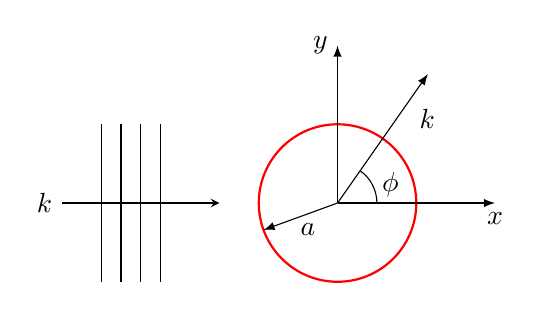
\begin{tikzpicture}
			\draw[red, thick] (0,0) circle (1);
			\draw[-latex] (0,0) -- ++(2,0) node[below] {$x$};
			\draw[-latex] (0,0) -- ++(0,2) node[left] {$y$};
			\draw[-latex] (0,0) -- node[pos=0.8, anchor=north west] {$\vect{k}$} (55:2);
			\draw (0,0) ++(0:0.5) arc (0:55:0.5) node[anchor=west, pos=0.5] {$\phi$};
			\draw[-latex] (0,0) -- node[below, pos=0.4] {$a$} ++(200:1);
			\draw foreach \i in {-3,-2.75,-2.5,-2.25} {(\i,1) -- (\i,-1) };
			\draw[-stealth] (-3.5, 0) node[left] {$\vect{k}$} -- ++(2,0);
		\end{tikzpicture}
		\captionof{figure}{До пояснення задачі}
	\end{center}

	Розглянемо випадок а) ($\Efield \parallel \vect{e}_z$).

	Поляризація, паралельна до осі циліндра, викликає поверхневі струми лише у напрямку осі $z$, а
	тому магнітного поля вздовж осі $z$ немає.
	%     $B_z = (\rot{\vect{A}})_z = 0$. З іншого боку $E_z = -\partial_z\pot - \partial_t A_z \neq
	%0$, таким чином, звідси випливає, що поза циліндром:
	%	\[
	%		B_{\phi} = -E_z.
	%	\]
	%
	%	Поляризація, перпендикулярна до осі циліндра індукує поверхневі струми в напрямку
	%$\vect{e}_{\phi}$, тому магнітне поле напрямлене вздовж осі $z$, а відповідно електричне поле
	%поза
	%межами циліндра (область хвиль) визначається як:
	%	\[
	%		B_z = E_{\phi}.
	%	\]

	Монохроматична плоска хвиля з частотою $\omega$ індукує  гармонічні струми і, як наслідок ми маємо
	розсіяну хвилю, яка теж є гармонічною.

	Поза циліндром електричне та магнітне поля задовольняють хвильовому рівнянню.
	Тому просторові частини $E_z$ і $B_z$ задовольняють рівнянню Гельмгольца:
	\[
		\left[ \Delta + \frac{\omega^2}{c^2}\right] u = 0,
	\]
	або в циліндричних координатах:
	\[
		\frac1r \frac{\partial }{\partial r}
		\left( r \frac{\partial u}{\partial r} \right) + \frac{1}{r^2} \frac{\partial^2 u}{\partial
		\phi^2} + k^2 u = 0.
	\]

	Розділимо змінні в останньому рівнянні $u(r,\phi) = R(r)G(\phi)$, одразу отримаємо $G(\phi) =
	e^{\pm im\phi}$, а рівняння для $R(r)$, як відомо, задовольняє рівняння диференціальному
	Бесселя~\eqref{eq:Bessel_eq}, якщо покласти $x = kr$:

	\begin{equation}\label{eq:BessProblem}\tag{*}
		\frac{d^2R}{dx^2} + \frac1x\frac{dR}{dx} + \left(1 - \frac{m^2}{x^2} \right) R = 0,
	\end{equation}
	розв'язок якого, як відомо, можна представити за допомогою функцій Бесселя $J_m(x)$ та Неймана
	$N_m$.
	%    Однак, оскільки для нашої задачі розсіяна хвиля має бути циліндричною при $r \to\infty$, тому
	В нашому випадку краще скористатись функціями Ганкеля 1-го роду, що дають асимптотику на
	нескінченності $e^{ikr}/\sqrt{r}$ (див.~\eqref{eq:Hxgg1}), яка відповідає умовам випромінювання.

	Поле  $E_z$ розсіяної хвилі будемо шукати як  лінійну комбінацію функцій $H_m^{(1)}e^{im\phi}$ з
	коефіцієнтами $A_m$:
	\[
		E_{z,\text{розс}} =  \sum\limits_{m = -\infty}^{\infty} A^m H^{(1)}_m(k r)e^{im\phi}.
	\]

	Поле плоскої падаючої хвилі $ E_{z,\text{пад}} = E_0e^{ikx} = E_0e^{ikr\cos\phi}$ розкладемо за
	функціями Бесселя (див~\eqref{eq:JacobiAnger}):
	\[
		E_{z,\text{пад}} =  E_0e^{ikr\cos\phi} =  E_0 \sum\limits_{m = -\infty}^{\infty} i^m J_m(k
		r)e^{im\phi}.
	\]

	Загальне поле є сумою падаючої та розсіяної хвиль, за принципом суперпозиції:
	\[
		E_z = E_0 \sum\limits_{m = -\infty}^{\infty}[ i^mJ_m(kr) + A_mH^{(1)}_m(kr)]e^{im\phi}.
	\]

	Далі скористаємось граничною умовою $E_z(r = a) = 0$  і визначимо $a_m$ з
	рівняння~\eqref{eq:BessProblem}; матимемо:
	\[
		E_z(r,\phi) = E_0e^{ikr\cos\phi} - E_0\sum\limits_{m = -\infty}^{\infty} i^m
		\frac{J_m(ka)}{H_m^{(1)}(ka)}H_m^{(1)}(kr)e^{im\phi}.
	\]

	Магнітне поле отримуємо з рівняння Максвелла $\Bfield = \frac1k\rot\Efield = \frac1k
	\vect{\nabla}E_z\times \vect{e}_z$,

	\[
		B_r=\frac{1}{kr}\frac{\partial E_z}{\partial \phi},
	\]
	\[
		B_\phi=-\frac{1}{k}\frac{\partial E_z}{\partial r}.
	\]

	Легко  перевірити, що $B_r=0$ при $r=a$ на  поверхні надпровідного циліндра і, таким чином,
	задовольняє граничній умові.

	Випадок б) ($\Efield \perp \vect{e}_z$).

	Для перпендикулярної поляризації викладки аналогічні, але тут зручніше починати з складової
	магнітного поля, яке у плоскій хвилі має вигляд $B_z = E_0e^{ikx}$. Гранична умова для
	тангенціальної компоненти електричного поля дає:
	\[
		E_{\phi}(r = a) = \left. \frac1k\frac{\partial B_z}{\partial r}\right|_{r = a} = 0.
	\]

	Отже
	\[
		B_z = E_0e^{ikr\cos\phi} - E_0\sum\limits_{m = -\infty}^{\infty} i^m
		\frac{J_m'(ka)}{H_m^{(1)\prime}(ka)}H_m^{(1)}(kr)e^{im\phi},
	\]
	де штрих <<$\prime$>> означає похідну по радіальній аргументу $kr$.

	Знайдемо тепер диференціальні перерізи розсіювання
	\(
	\frac{d\sigma}{d\phi} = r \frac{|\Efield_\text{розс}|^2}{|\Efield_\text{пад}|^2}
	\).

	Враховуючи, що$\lim\limits_{r\to\infty}H_m^{(1)}(kr) = \sqrt{\frac{2}{\pi k r}}$, маємо:
	\[
		\frac{d\sigma_{\parallel}}{d\phi} = \frac{2}{\pi k} \left| \sum\limits_{m = -\infty}^{\infty}
		\frac{J_m(ka)}{H_m^{(1)}(ka)}e^{im\phi} \right|^2, \quad
		\frac{d\sigma_{\perp}}{d\phi} = \frac{2}{\pi k} \left| \sum\limits_{m = -\infty}^{\infty}
		\frac{J_m(ka)'}{H_m^{(1)\prime}(ka)}e^{im\phi} \right|^2.
	\]

	Ці диференціальні перерізи мають розмірність довжини (а не площі), оскільки вони визначають
	потужність на одиницю довжини циліндра, тобто потужність, випромінювана через границю великого
	кола, співвісного з циліндром.

	Повні перерізи:
	\[
		\sigma_{\parallel} = \frac4k \sum\limits_{m = -\infty}^{\infty} \frac{J_m^2(ka)}{J_m^2(ka) +
		N_m^2(ka)}, \quad
		\sigma_{\perp} = \frac4k \sum\limits_{m = -\infty}^{\infty}
		\frac{J_m^{2\prime}(ka)}{J_m^{2\prime}(ka) + N_m^{2\prime}(ka)}.
	\]
\end{solution}
\end{problem}

%=========================================================
\begin{problem}%Zangwill 21.9
Поляризоване монохроматичне світло, хвильовий вектор якого $\vect{k}_0$  і амплітуда $E_0$ нормально
падає з вакууму на бічну поверхню нескінченно довгого діелектричного циліндра радіуса $a$ з
проникністю $\epsilon$ (для даної частоти). Знайдіть електричне поле у всьому просторі, якщо напрямок
поляризації світла паралельний до осі симетрії циліндра.
\begin{solution}
	На рисунку показана плоска хвиля, яка поширюється в напрямку $x$ перпендикулярно до діелектричного
	циліндра, вісь якого напрямлена вздовж осі $z$.

	\begin{center}
		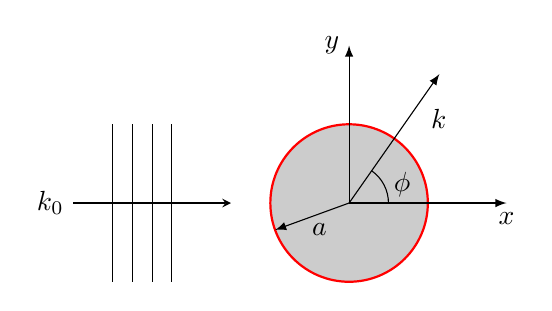
\begin{tikzpicture}
			\draw[red, thick, fill=gray!40] (0,0) circle (1);
			\draw[-latex] (0,0) -- ++(2,0) node[below] {$x$};
			\draw[-latex] (0,0) -- ++(0,2) node[left] {$y$};
			\draw[-latex] (0,0) -- node[pos=0.8, anchor=north west] {$\vect{k}$} (55:2);
			\draw (0,0) ++(0:0.5) arc (0:55:0.5) node[anchor=west, pos=0.5] {$\phi$};
			\draw[-latex] (0,0) -- node[below, pos=0.4] {$a$} ++(200:1);
			\draw foreach \i in {-3,-2.75,-2.5,-2.25} {(\i,1) -- (\i,-1) };
			\draw[-stealth] (-3.5, 0) node[left] {$\vect{k}_0$} -- ++(2,0);
		\end{tikzpicture}
		\captionof{figure}{До пояснення задачі}
	\end{center}

	Вказівка: дивіться розв'язок задачі~\ref{prb:Zang_metall_Cyllinder} і врахуйте необхідну
	поляризацію, та граничні умови для поля на межі розділу.

	Поле в циліндрі $r < a$ шукаємо у вигляді:
	\[
		E_{z,\text{in}} = \sum\limits_{m = -\infty}^{\infty}A_mJ_m(kr)e^{im\phi}, \quad
		k=\sqrt{\epsilon} \omega/c.
	\]

	Зовні, електричне поле є сумою падаючої та розсіяної хвилі:
	\[
		E_z = E_0 \sum\limits_{m = -\infty}^{\infty} \left( i^m J_m(k_0 r) + B_m H_m^{(1)(k_0r)}
		\right) e^{im\phi}, \quad k= \omega/c.
	\]
	де
	\[
		A_m = E_0i^m \frac{  H_m^{(1)}(k_0a) J'_m(k_0a) - H_m^{(1)\prime}(k_0a) J_m(k_0a)    }{
		\sqrt{\epsilon} H_m^{(1)}(k_0a) J'_m(ka) - H_m^{(1)\prime}(k_0a) J_m(ka)},
	\]
	\[
		B_m = E_0i^m \frac{  J_m(ka) J'_m(k_0a) - \sqrt{\epsilon} J_m'(ka) J_m(k_0a)    }{
		\sqrt{\epsilon} H_m^{(1)}(k_0a) J'_m(ka) - H_m^{(1)\prime}(k_0a) J_m(ka)}.
	\]

\end{solution}
\end{problem}

\begin{problem}
Запишіть диференціальний і повний перерізи розсіювання природного монохроматичного світла довжиною
$\lambda$ на металевій сфері радіуса $R \ll \lambda$.
\begin{solution}
	За умови задачі  електричне і магнітне поля хвилі, які можна вважати квазистаціонарними, індукують
	в надпровідній кулі електричний дипольний момент $p_e=ER^3$ та магнітний момент $p_m=-BR^{3/2}$.
	Звідси отримуємо сумарне магнітне поле в хвильовій зоні за формулами дипольного та
	магнітодипольного випромінювання.
	Диференціальний переріз
	\[
		\frac{d\sigma}{do} = R^6 k^4 \left[\frac58 (1 + \cos^2\theta) -\cos\theta\right],
	\]
	де $k$~--- хвильове число, $\theta = \widehat{\vect{k}_0,\vect{k}}$~--- кут між напрямками
	падаючої та розсіяної хвилі.
	Повний переріз $\sigma = \frac{10\pi R^6 k^4}{3}$.
\end{solution}
\end{problem}

%=========================================================
\begin{problem}[Дифракція Фраунгофера]
Плоска хвиля, яка падає нормально на площину, проходить через невеликий прямокутний отвір сторонами
$a$ та $b$, який вирізано в цій площині згідно умов $|x|< a$, $|y|<b$. Знайти розподіл інтенсивності
на поверхні, що знаходиться на відстані $l$ від площини.
\begin{solution}
	$I(x,y) = I_0\frac{\sin^2\alpha}{\alpha^2}\frac{\sin^2\beta}{\beta^2}$, де $\alpha =
	\frac{kax}{2l}$, $\beta=\frac{kby}{2l}$.
\end{solution}
\end{problem}

%=========================================================
\begin{problem}
Плоска хвиля, яка падає нормально на площину, проходить через невеликий круглий отвір радіусом $R$,
який вирізано в цій площині. Знайти розподіл інтенсивності на поверхні, що знаходиться на відстані $l$
від площини.
\begin{solution}
	Вказівка: при інтегруванні слід врахувати співвідношення для функцій Бесселя~\eqref{eq:recInt}
	$\int\limits_0^x x'J_0(x')dx' = xJ_1(x)$.

	Відповідь: $I(r) = 4I_0\left( \frac{J_1\left( \frac{kRr}{l}\right) }{\frac{kRr}{l}}\right)^2$.
\end{solution}
\end{problem}

%=========================================================
\begin{problem}[Дифракція Френеля]
Оцінити наближений розподіл інтенсивності на площині екрану, розташованого при $z = D$   при дифракції
на напівплощині ($z = 0$, нормальне падіння) далеко в області тіні.
\end{problem}

%=========================================================
\begin{problem}[Геометрична оптика]
Знайти кут відхилення променя у середовищі із коефіцієнтом заломлення $n = 1 - \frac{a}{r}$. Промінь
проходить в області, де  $\frac{a}{r} \ll 1$. Прицільна відстань відносно початку координат $b$.
\end{problem}

\Closesolutionfile{answer}

